% Options for packages loaded elsewhere
\PassOptionsToPackage{unicode}{hyperref}
\PassOptionsToPackage{hyphens}{url}
%
\documentclass[
  english,
  man,floatsintext]{apa7}
\usepackage{amsmath,amssymb}
\usepackage{lmodern}
\usepackage{ifxetex,ifluatex}
\ifnum 0\ifxetex 1\fi\ifluatex 1\fi=0 % if pdftex
  \usepackage[T1]{fontenc}
  \usepackage[utf8]{inputenc}
  \usepackage{textcomp} % provide euro and other symbols
\else % if luatex or xetex
  \usepackage{unicode-math}
  \defaultfontfeatures{Scale=MatchLowercase}
  \defaultfontfeatures[\rmfamily]{Ligatures=TeX,Scale=1}
\fi
% Use upquote if available, for straight quotes in verbatim environments
\IfFileExists{upquote.sty}{\usepackage{upquote}}{}
\IfFileExists{microtype.sty}{% use microtype if available
  \usepackage[]{microtype}
  \UseMicrotypeSet[protrusion]{basicmath} % disable protrusion for tt fonts
}{}
\makeatletter
\@ifundefined{KOMAClassName}{% if non-KOMA class
  \IfFileExists{parskip.sty}{%
    \usepackage{parskip}
  }{% else
    \setlength{\parindent}{0pt}
    \setlength{\parskip}{6pt plus 2pt minus 1pt}}
}{% if KOMA class
  \KOMAoptions{parskip=half}}
\makeatother
\usepackage{xcolor}
\IfFileExists{xurl.sty}{\usepackage{xurl}}{} % add URL line breaks if available
\IfFileExists{bookmark.sty}{\usepackage{bookmark}}{\usepackage{hyperref}}
\hypersetup{
  pdftitle={Appendix},
  pdflang={en-EN},
  hidelinks,
  pdfcreator={LaTeX via pandoc}}
\urlstyle{same} % disable monospaced font for URLs
\usepackage{graphicx}
\makeatletter
\def\maxwidth{\ifdim\Gin@nat@width>\linewidth\linewidth\else\Gin@nat@width\fi}
\def\maxheight{\ifdim\Gin@nat@height>\textheight\textheight\else\Gin@nat@height\fi}
\makeatother
% Scale images if necessary, so that they will not overflow the page
% margins by default, and it is still possible to overwrite the defaults
% using explicit options in \includegraphics[width, height, ...]{}
\setkeys{Gin}{width=\maxwidth,height=\maxheight,keepaspectratio}
% Set default figure placement to htbp
\makeatletter
\def\fps@figure{htbp}
\makeatother
\setlength{\emergencystretch}{3em} % prevent overfull lines
\providecommand{\tightlist}{%
  \setlength{\itemsep}{0pt}\setlength{\parskip}{0pt}}
\setcounter{secnumdepth}{5}
% Make \paragraph and \subparagraph free-standing
\ifx\paragraph\undefined\else
  \let\oldparagraph\paragraph
  \renewcommand{\paragraph}[1]{\oldparagraph{#1}\mbox{}}
\fi
\ifx\subparagraph\undefined\else
  \let\oldsubparagraph\subparagraph
  \renewcommand{\subparagraph}[1]{\oldsubparagraph{#1}\mbox{}}
\fi
% Manuscript styling
\usepackage{upgreek}
\captionsetup{font=singlespacing,justification=justified}

% Table formatting
\usepackage{longtable}
\usepackage{lscape}
% \usepackage[counterclockwise]{rotating}   % Landscape page setup for large tables
\usepackage{multirow}		% Table styling
\usepackage{tabularx}		% Control Column width
\usepackage[flushleft]{threeparttable}	% Allows for three part tables with a specified notes section
\usepackage{threeparttablex}            % Lets threeparttable work with longtable

% Create new environments so endfloat can handle them
% \newenvironment{ltable}
%   {\begin{landscape}\begin{center}\begin{threeparttable}}
%   {\end{threeparttable}\end{center}\end{landscape}}
\newenvironment{lltable}{\begin{landscape}\begin{center}\begin{ThreePartTable}}{\end{ThreePartTable}\end{center}\end{landscape}}

% Enables adjusting longtable caption width to table width
% Solution found at http://golatex.de/longtable-mit-caption-so-breit-wie-die-tabelle-t15767.html
\makeatletter
\newcommand\LastLTentrywidth{1em}
\newlength\longtablewidth
\setlength{\longtablewidth}{1in}
\newcommand{\getlongtablewidth}{\begingroup \ifcsname LT@\roman{LT@tables}\endcsname \global\longtablewidth=0pt \renewcommand{\LT@entry}[2]{\global\advance\longtablewidth by ##2\relax\gdef\LastLTentrywidth{##2}}\@nameuse{LT@\roman{LT@tables}} \fi \endgroup}

% \setlength{\parindent}{0.5in}
% \setlength{\parskip}{0pt plus 0pt minus 0pt}

% Overwrite redefinition of paragraph and subparagraph by the default LaTeX template
% See https://github.com/crsh/papaja/issues/292
\makeatletter
\renewcommand{\paragraph}{\@startsection{paragraph}{4}{\parindent}%
  {0\baselineskip \@plus 0.2ex \@minus 0.2ex}%
  {-1em}%
  {\normalfont\normalsize\bfseries\itshape\typesectitle}}

\renewcommand{\subparagraph}[1]{\@startsection{subparagraph}{5}{1em}%
  {0\baselineskip \@plus 0.2ex \@minus 0.2ex}%
  {-\z@\relax}%
  {\normalfont\normalsize\itshape\hspace{\parindent}{#1}\textit{\addperi}}{\relax}}
\makeatother

% \usepackage{etoolbox}
\makeatletter
\patchcmd{\HyOrg@maketitle}
  {\section{\normalfont\normalsize\abstractname}}
  {\section*{\normalfont\normalsize\abstractname}}
  {}{\typeout{Failed to patch abstract.}}
\patchcmd{\HyOrg@maketitle}
  {\section{\protect\normalfont{\@title}}}
  {\section*{\protect\normalfont{\@title}}}
  {}{\typeout{Failed to patch title.}}
\makeatother
\shorttitle{}
\usepackage{csquotes}
\usepackage[export]{adjustbox}
\usepackage{makecell}
\renewcommand{\cellset}{\renewcommand{\arraystretch}{0.7}}
\ifxetex
  % Load polyglossia as late as possible: uses bidi with RTL langages (e.g. Hebrew, Arabic)
  \usepackage{polyglossia}
  \setmainlanguage[]{english}
\else
  \usepackage[main=english]{babel}
% get rid of language-specific shorthands (see #6817):
\let\LanguageShortHands\languageshorthands
\def\languageshorthands#1{}
\fi
\ifluatex
  \usepackage{selnolig}  % disable illegal ligatures
\fi

\title{Appendix}
\author{\textsuperscript{}}
\date{}


\affiliation{\vspace{0.5cm}\textsuperscript{} }

\begin{document}
\maketitle

\hypertarget{appendix-a}{%
\section*{Appendix A}\label{appendix-a}}
\addcontentsline{toc}{section}{Appendix A}

\setcounter{table}{0}
\renewcommand{\thetable}{A\arabic{table}}

\begin{center}
\begin{ThreePartTable}

\footnotesize{

\begin{longtable}{llll}\noalign{\getlongtablewidth\global\LTcapwidth=\longtablewidth}
\caption{\label{tab:appendix}Unfamiliar Object Stimuli\smallskip}\\
\toprule
Picture & ID & Matching keywords & Non-matching keywords\\
\midrule
\endfirsthead
\caption*{\normalfont{Table \ref{tab:appendix} continued}}\\
\toprule
Picture & ID & Matching keywords & Non-matching keywords\\
\midrule
\endhead
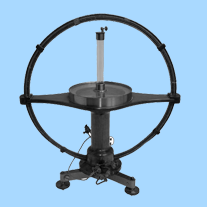
\includegraphics[valign=c, scale=0.23]{../materials/unfamiliar/1.png} & 1 & \makecell[l]{elektrische Spannung, prüfen\\{[electric current, measuring]}} & \makecell[l]{Makkaroni, formen\\{[macaroni, forming]}}\\
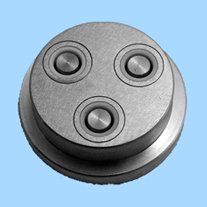
\includegraphics[valign=c, scale=0.23]{../materials/unfamiliar/2.png} & 2 & \makecell[l]{Makkaroni, formen\\{[macaroni, forming]}} & \makecell[l]{Kuh, vom Zaun abhalten\\{[cow, keeping away from the fence]}}\\
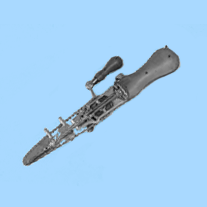
\includegraphics[valign=c, scale=0.23]{../materials/unfamiliar/3.png} & 3 & \makecell[l]{Knochen, sägen\\{[bones, sawing]}} & \makecell[l]{Streckenmaß, Sonnenlicht nutzen\\{[distance measure, using sunrays]}}\\
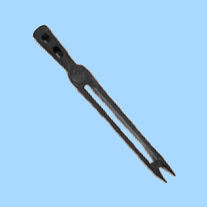
\includegraphics[valign=c, scale=0.23]{../materials/unfamiliar/4.png} & 4 & \makecell[l]{Unkraut, jäten\\{[weed, removing]}} & \makecell[l]{Uhr, mit Wärme betreiben\\{[clock, operating with heat]}}\\
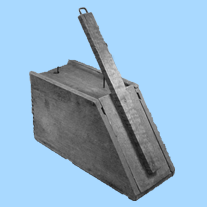
\includegraphics[valign=c, scale=0.23]{../materials/unfamiliar/5.png} & 5 & \makecell[l]{Mausefalle, zuschnappen\\{[mousetrap, snap-shutting]}} & \makecell[l]{Brillenglas, zuschneiden\\{[eyeglass lense, cutting]}}\\
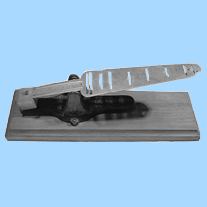
\includegraphics[valign=c, scale=0.23]{../materials/unfamiliar/6.png} & 6 & \makecell[l]{Goldmünzen, wiegen\\{[gold coin, weighing]}} & \makecell[l]{Farbe, vom Fenster abschleifen\\{[paint, scraping off the window]}}\\
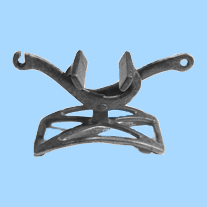
\includegraphics[valign=c, scale=0.23]{../materials/unfamiliar/7.png} & 7 & \makecell[l]{Knie, fixieren\\{[knee, fixating]}} & \makecell[l]{Buchstaben, tippen\\{[letter, typing]}}\\
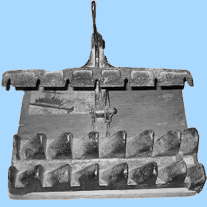
\includegraphics[valign=c, scale=0.23]{../materials/unfamiliar/8.png} & 8 & \makecell[l]{Eierkarton, pressen\\{[egg carton, pressing]}} & \makecell[l]{Tabak, zermahlen\\{[tobacco, pulverize]}}\\
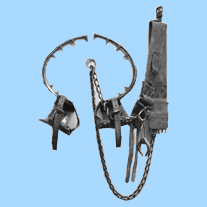
\includegraphics[valign=c, scale=0.23]{../materials/unfamiliar/9.png} & 9 & \makecell[l]{Baum, erklettern\\{[tree, climbing]}} & \makecell[l]{Rotation, Ladung erzeugen\\{[rotation, creating electric charge]}}\\
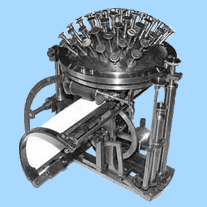
\includegraphics[valign=c, scale=0.23]{../materials/unfamiliar/10.png} & 10 & \makecell[l]{Buchstaben, tippen\\{[letter, typing]}} & \makecell[l]{Pferdehuf, Halt geben\\{[horse hoof, giving grip]}}\\
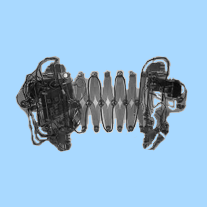
\includegraphics[valign=c, scale=0.23]{../materials/unfamiliar/11.png} & 11 & \makecell[l]{Akkordeon, spielen\\{[accordion, playing]}} & \makecell[l]{Seil, schneiden\\{[rope, cutting]}}\\
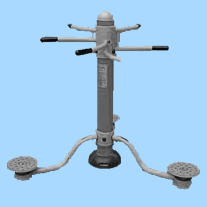
\includegraphics[valign=c, scale=0.23]{../materials/unfamiliar/12.png} & 12 & \makecell[l]{Körper, trainieren\\{[body, training]}} & \makecell[l]{Buch, offen halten\\{[book, binding]}}\\
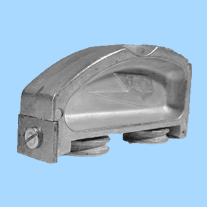
\includegraphics[valign=c, scale=0.23]{../materials/unfamiliar/13.png} & 13 & \makecell[l]{Farbe, vom Fenster abschleifen\\{[paint, scraping off the window]}} & \makecell[l]{von Hand, zentrifugieren\\{[by hand, centrifugating]}}\\
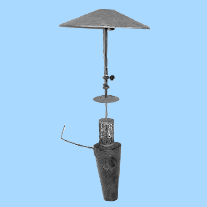
\includegraphics[valign=c, scale=0.23]{../materials/unfamiliar/14.png} & 14 & \makecell[l]{Außenbereich, heizen\\{[outdoor area, heating]}} & \makecell[l]{Rasierklinge, schärfen\\{[razor blade, sharpening]}}\\
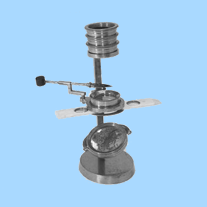
\includegraphics[valign=c, scale=0.23]{../materials/unfamiliar/15.png} & 15 & \makecell[l]{Pflanzenteile, vergrößern\\{[plant parts, magnifying]}} & \makecell[l]{Katzenklo, sich selbst reinigen\\{[litter box, self-cleaning]}}\\
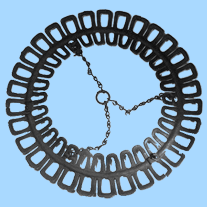
\includegraphics[valign=c, scale=0.23]{../materials/unfamiliar/16.png} & 16 & \makecell[l]{Krawatten, aufhängen\\{[necktie, hanging up]}} & \makecell[l]{Zeichnungen, vermessen\\{[drawings, measuring]}}\\
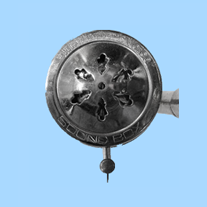
\includegraphics[valign=c, scale=0.23]{../materials/unfamiliar/17.png} & 17 & \makecell[l]{Schallplatte, abtasten\\{[vinyl record, reading]}} & \makecell[l]{Ball, katapultieren\\{[ball, catapulting]}}\\
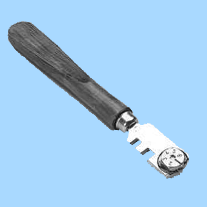
\includegraphics[valign=c, scale=0.23]{../materials/unfamiliar/18.png} & 18 & \makecell[l]{Glas, schneiden\\{[glass, cutting]}} & \makecell[l]{Eier, wiegen\\{[eggs, weighing]}}\\
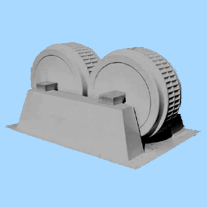
\includegraphics[valign=c, scale=0.23]{../materials/unfamiliar/19.png} & 19 & \makecell[l]{Briketts, pressen\\{[briquette, pressing]}} & \makecell[l]{Narkosemittel, abgeben\\{[anesthetic, administering]}}\\
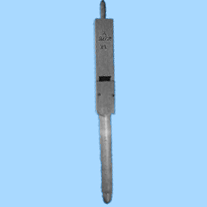
\includegraphics[valign=c, scale=0.23]{../materials/unfamiliar/20.png} & 20 & \makecell[l]{Orgelton, erzeugen\\{[organ sound, making]}} & \makecell[l]{Bandage, rollen\\{[bandage, rolling]}}\\
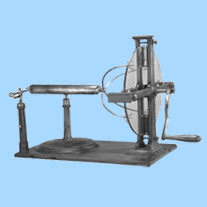
\includegraphics[valign=c, scale=0.23]{../materials/unfamiliar/21.png} & 21 & \makecell[l]{Spannung, erzeugen\\{[electric current, making]}} & \makecell[l]{Fußstütze, reiten\\{[footrest, horseback riding]}}\\
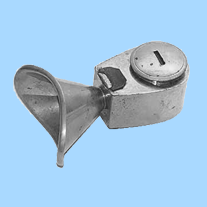
\includegraphics[valign=c, scale=0.23]{../materials/unfamiliar/22.png} & 22 & \makecell[l]{Narkosemittel, abgeben\\{[anesthetic, administering]}} & \makecell[l]{Nüsse, aufbrechen\\{[nuts, cracking]}}\\
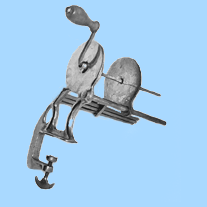
\includegraphics[valign=c, scale=0.23]{../materials/unfamiliar/23.png} & 23 & \makecell[l]{Bandage, rollen\\{[bandage, rolling]}} & \makecell[l]{Schnee, rodeln\\{[snow, sleighing]}}\\
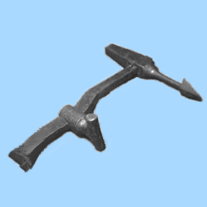
\includegraphics[valign=c, scale=0.23]{../materials/unfamiliar/24.png} & 24 & \makecell[l]{Weinfass, Loch einschlagen\\{[wine barrel, smashing a hole]}} & \makecell[l]{Tier, einfangen\\{[animal, trapping]}}\\
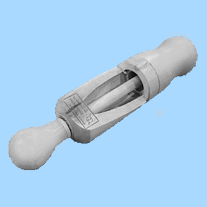
\includegraphics[valign=c, scale=0.23]{../materials/unfamiliar/25.png} & 25 & \makecell[l]{Flaschenkorken, einführen\\{[bottle cork, inserting]}} & \makecell[l]{Pferd, im Moor laufen\\{[horse, walking in the moor]}}\\
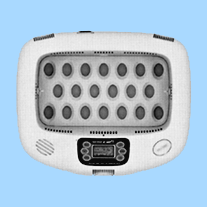
\includegraphics[valign=c, scale=0.23]{../materials/unfamiliar/26.png} & 26 & \makecell[l]{Automat, Eier ausbrüten\\{[machine, incubating eggs]}} & \makecell[l]{Windgeschwindigkeit, messen\\{[wind speed, measuring]}}\\
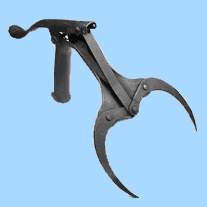
\includegraphics[valign=c, scale=0.23]{../materials/unfamiliar/27.png} & 27 & \makecell[l]{Korngarbe, greifen\\{[sheaf, grabbing]}} & \makecell[l]{Treibhaus, heizen\\{[glass house, heating]}}\\
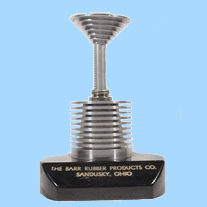
\includegraphics[valign=c, scale=0.23]{../materials/unfamiliar/28.png} & 28 & \makecell[l]{Brief, wiegen\\{[letter, weighing]}} & \makecell[l]{Korngarbe, greifen\\{[sheaf, grabbing]}}\\
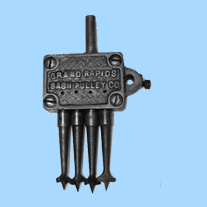
\includegraphics[valign=c, scale=0.23]{../materials/unfamiliar/29.png} & 29 & \makecell[l]{Löcher, bohren\\{[hole, drilling]}} & \makecell[l]{Sonnenlicht, Intensität messen\\{[sunlight, measure intensity]}}\\
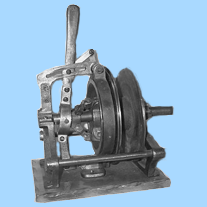
\includegraphics[valign=c, scale=0.23]{../materials/unfamiliar/30.png} & 30 & \makecell[l]{Angelschnur, kurbeln\\{[fishing line, winding]}} & \makecell[l]{Glaskörper, musizieren\\{[glass body, making music]}}\\
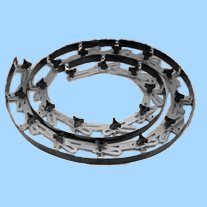
\includegraphics[valign=c, scale=0.23]{../materials/unfamiliar/31.png} & 31 & \makecell[l]{Kurven, malen\\{[curve, drawing]}} & \makecell[l]{Nussöl, pressen\\{[nut oil, pressing]}}\\
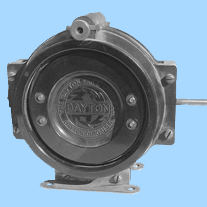
\includegraphics[valign=c, scale=0.23]{../materials/unfamiliar/32.png} & 32 & \makecell[l]{Radiofrequenz, einstellen\\{[radio frequency, tuning]}} & \makecell[l]{Erektion, helfen\\{[erection, helping]}}\\
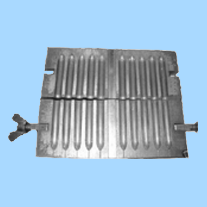
\includegraphics[valign=c, scale=0.23]{../materials/unfamiliar/33.png} & 33 & \makecell[l]{Zäpfchen, pressen\\{[suppository, pressing]}} & \makecell[l]{Unkraut, jäten\\{[weed, removing]}}\\
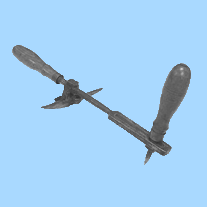
\includegraphics[valign=c, scale=0.23]{../materials/unfamiliar/34.png} & 34 & \makecell[l]{Fass, öffnen\\{[barrel, opening]}} & \makecell[l]{Pflanzenteile, vergrößern\\{[plant parts, magnifying]}}\\
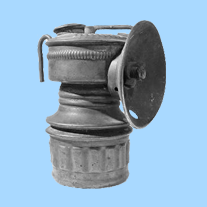
\includegraphics[valign=c, scale=0.23]{../materials/unfamiliar/35.png} & 35 & \makecell[l]{Bergbaustollen, beleuchten\\{[mining tunnel, lightening]}} & \makecell[l]{Knie, fixieren\\{[knee, fixating]}}\\
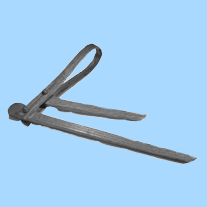
\includegraphics[valign=c, scale=0.23]{../materials/unfamiliar/36.png} & 36 & \makecell[l]{Kuh, vom Zaun abhalten\\{[cow, keeping away from the fence]}} & \makecell[l]{Radiofrequenz, einstellen\\{[radio frequency, tuning]}}\\
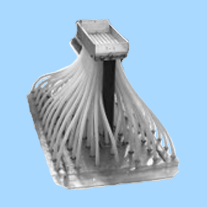
\includegraphics[valign=c, scale=0.23]{../materials/unfamiliar/37.png} & 37 & \makecell[l]{Saatgut, gleichmäßig aussäen\\{[seeds, sowing evenly]}} & \makecell[l]{Fass, öffnen\\{[barrel, opening]}}\\
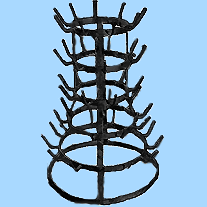
\includegraphics[valign=c, scale=0.23]{../materials/unfamiliar/38.png} & 38 & \makecell[l]{Flaschen, trocknen\\{[bottles, drying]}} & \makecell[l]{Bleistift, anspitzen\\{[pencil, sharpening]}}\\
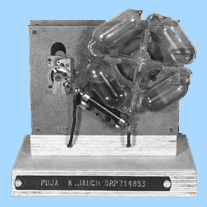
\includegraphics[valign=c, scale=0.23]{../materials/unfamiliar/39.png} & 39 & \makecell[l]{Uhr, mit Wärme betreiben\\{[clock, operating with heat]}} & \makecell[l]{Körper, untersuchen\\{[body, training]}}\\
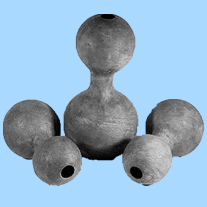
\includegraphics[valign=c, scale=0.23]{../materials/unfamiliar/40.png} & 40 & \makecell[l]{Tonpott, trommeln\\{[clay pot, drumming]}} & \makecell[l]{Piano, stimmen\\{[piano, tuning]}}\\
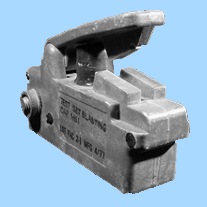
\includegraphics[valign=c, scale=0.23]{../materials/unfamiliar/41.png} & 41 & \makecell[l]{Sprengstoffexplosion, auslösen\\{[dynamite explosion, triggering]}} & \makecell[l]{Fisch, wiegen\\{[fish, weighing]}}\\
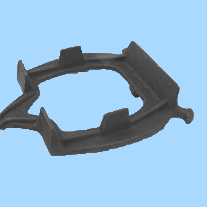
\includegraphics[valign=c, scale=0.23]{../materials/unfamiliar/42.png} & 42 & \makecell[l]{Pferdehuf, Halt geben\\{[horse hoof, giving grip]}} & \makecell[l]{Zäpfchen, pressen\\{[suppository, pressing]}}\\
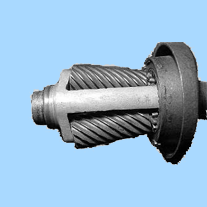
\includegraphics[valign=c, scale=0.23]{../materials/unfamiliar/43.png} & 43 & \makecell[l]{Bleistift, anspitzen\\{[pencil, sharpening]}} & \makecell[l]{Angel, Köder markieren\\{[fishing rod, marking bait]}}\\
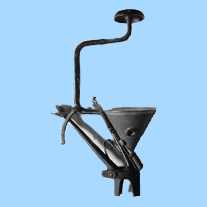
\includegraphics[valign=c, scale=0.23]{../materials/unfamiliar/44.png} & 44 & \makecell[l]{Nussöl, pressen\\{[nut oil, pressing]}} & \makecell[l]{Zeichen, einbrennen\\{[marks, burning in]}}\\
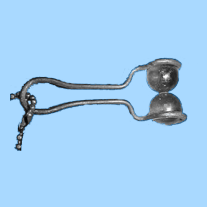
\includegraphics[valign=c, scale=0.23]{../materials/unfamiliar/45.png} & 45 & \makecell[l]{Rasierklinge, schärfen\\{[razor blade, sharpening]}} & \makecell[l]{Kurven, malen\\{[curve, drawing]}}\\
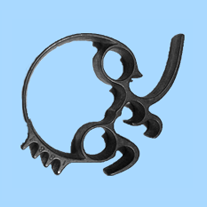
\includegraphics[valign=c, scale=0.23]{../materials/unfamiliar/46.png} & 46 & \makecell[l]{heiße Platten, anheben\\{[hot plates, lifting]}} & \makecell[l]{Kleidung, im Eimer waschen\\{[clothes, washing in a bucket]}}\\
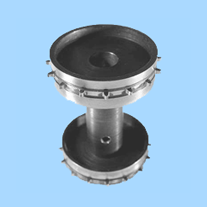
\includegraphics[valign=c, scale=0.23]{../materials/unfamiliar/47.png} & 47 & \makecell[l]{Film, aufspulen\\{[film roll, winding]}} & \makecell[l]{Mund, offen halten\\{[mouth, keeping open]}}\\
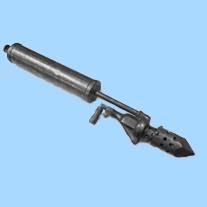
\includegraphics[valign=c, scale=0.23]{../materials/unfamiliar/48.png} & 48 & \makecell[l]{Waffe, entflammen\\{[weapon, inflaming]}} & \makecell[l]{Uhrzeit, anzeigen\\{[time, displaying]}}\\
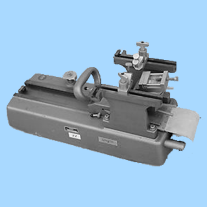
\includegraphics[valign=c, scale=0.23]{../materials/unfamiliar/49.png} & 49 & \makecell[l]{Mikroskop-Proben, schneiden\\{[microscopic samples, slicing]}} & \makecell[l]{heiße Platten, anheben\\{[hot plates, lifting]}}\\
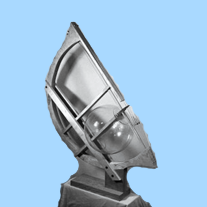
\includegraphics[valign=c, scale=0.23]{../materials/unfamiliar/50.png} & 50 & \makecell[l]{Glaskörper, musizieren\\{[glass body, making music]}} & \makecell[l]{Kork, flach pressen\\{[cork, pressing flat]}}\\
\includegraphics[valign=c, scale=0.23]{../materials/unfamiliar/51.png} & 51 & \makecell[l]{Dampf, zerstäuben\\{[steam, spraying]}} & \makecell[l]{Buch, binden\\{[book, opening]}}\\
\includegraphics[valign=c, scale=0.23]{../materials/unfamiliar/52.png} & 52 & \makecell[l]{Mandeln, operieren\\{[kidneys, operating]}} & \makecell[l]{Film, aufspulen\\{[film roll, winding]}}\\
\includegraphics[valign=c, scale=0.23]{../materials/unfamiliar/53.png} & 53 & \makecell[l]{Toastbrot, rösten\\{[toast, roasting]}} & \makecell[l]{Autobatterie, Spannung testen\\{[car battery, measuring voltage]}}\\
\includegraphics[valign=c, scale=0.23]{../materials/unfamiliar/54.png} & 54 & \makecell[l]{Fußstütze, reiten\\{[footrest, horseback riding]}} & \makecell[l]{Stromstärke, messen\\{[current, measuring]}}\\
\includegraphics[valign=c, scale=0.23]{../materials/unfamiliar/55.png} & 55 & \makecell[l]{Türgelenk, Feuer überstehen\\{[door hinge, survining fires]}} & \makecell[l]{Botschaft, telegrafieren\\{[message, telegraphing]}}\\
\includegraphics[valign=c, scale=0.23]{../materials/unfamiliar/56.png} & 56 & \makecell[l]{Schnee, rodeln\\{[snow, sleighing]}} & \makecell[l]{Dampf, zerstäuben\\{[steam, spraying]}}\\
\includegraphics[valign=c, scale=0.23]{../materials/unfamiliar/57.png} & 57 & \makecell[l]{Nüsse, aufbrechen\\{[nuts, cracking]}} & \makecell[l]{Ziegelsteine, formen\\{[bricks, forming]}}\\
\includegraphics[valign=c, scale=0.23]{../materials/unfamiliar/58.png} & 58 & \makecell[l]{Radiergummi, mit Strom betreiben\\{[eraser, operating with electricity]}} & \makecell[l]{Münzen, aufbewahren\\{[coins, storing]}}\\
\includegraphics[valign=c, scale=0.23]{../materials/unfamiliar/59.png} & 59 & \makecell[l]{Treibhaus, heizen\\{[glass house, heating]}} & \makecell[l]{Messer, schleifen\\{[knife, sharpening]}}\\
\includegraphics[valign=c, scale=0.23]{../materials/unfamiliar/60.png} & 60 & \makecell[l]{Botschaft, telegrafieren\\{[message, telegraphing]}} & \makecell[l]{Toastbrot, rösten\\{[toast, roasting]}}\\
\includegraphics[valign=c, scale=0.23]{../materials/unfamiliar/61.png} & 61 & \makecell[l]{Angel, Köder markieren\\{[fishing rod, marking bait]}} & \makecell[l]{Baum, erklettern\\{[tree, climbing]}}\\
\includegraphics[valign=c, scale=0.23]{../materials/unfamiliar/62.png} & 62 & \makecell[l]{Katzenklo, sich selbst reinigen\\{[litter box, self-cleaning]}} & \makecell[l]{Tankfüllstand, messen\\{[fuel tank level, gauging]}}\\
\includegraphics[valign=c, scale=0.23]{../materials/unfamiliar/63.png} & 63 & \makecell[l]{Körper, untersuchen\\{[body, examining]}} & \makecell[l]{Schuhe, auf Eis laufen\\{[shoes, walking on ice]}}\\
\includegraphics[valign=c, scale=0.23]{../materials/unfamiliar/64.png} & 64 & \makecell[l]{Brillenglas, zuschneiden\\{[eyeglass lense, cutting]}} & \makecell[l]{Saatgut, gleichmäßig aussäen\\{[seeds, sowing evenly]}}\\
\includegraphics[valign=c, scale=0.23]{../materials/unfamiliar/65.png} & 65 & \makecell[l]{Draht, wickeln\\{[wire, winding]}} & \makecell[l]{Bergbaustollen, beleuchten\\{[mining tunnel, lightening]}}\\
\includegraphics[valign=c, scale=0.23]{../materials/unfamiliar/66.png} & 66 & \makecell[l]{Buch, offen halten\\{[book, opening]}} & \makecell[l]{Sprengstoffexplosion, auslösen\\{[dynamite explosion, triggering]}}\\
\includegraphics[valign=c, scale=0.23]{../materials/unfamiliar/67.png} & 67 & \makecell[l]{Feldanbau, häckseln\\{[harvest, chopping]}} & \makecell[l]{Draht, wickeln\\{[wire, winding]}}\\
\includegraphics[valign=c, scale=0.23]{../materials/unfamiliar/68.png} & 68 & \makecell[l]{Schnurlot, absenken\\{[plummet, letting down]}} & \makecell[l]{Korken, formen\\{[bottle cork, forming]}}\\
\includegraphics[valign=c, scale=0.23]{../materials/unfamiliar/69.png} & 69 & \makecell[l]{Sternenbilder, vermessen\\{[stellar constellation, measuring]}} & \makecell[l]{Schnurlot, absenken\\{[plummet, letting down]}}\\
\includegraphics[valign=c, scale=0.23]{../materials/unfamiliar/70.png} & 70 & \makecell[l]{Nachricht, morsen\\{[message, signalling]}} & \makecell[l]{Feldanbau, häckseln\\{[harvest, chopping]}}\\
\includegraphics[valign=c, scale=0.23]{../materials/unfamiliar/71.png} & 71 & \makecell[l]{Musikgerät, stampfen\\{[musical instrument, stamping]}} & \makecell[l]{Goldmünzen, wiegen\\{[gold coin, weighing]}}\\
\includegraphics[valign=c, scale=0.23]{../materials/unfamiliar/72.png} & 72 & \makecell[l]{Schuhe, auf Eis laufen\\{[shoes, walking on ice]}} & \makecell[l]{Geschwindigkeit, ermitteln\\{[speed, determining]}}\\
\includegraphics[valign=c, scale=0.23]{../materials/unfamiliar/73.png} & 73 & \makecell[l]{Geschwindigkeit, ermitteln\\{[speed, determining]}} & \makecell[l]{Mausefalle, zuschnappen\\{[mousetrap, snap-shutting]}}\\
\includegraphics[valign=c, scale=0.23]{../materials/unfamiliar/74.png} & 74 & \makecell[l]{Zeichen, einbrennen\\{[marks, burning in]}} & \makecell[l]{Luftdruck, messen\\{[air pressure, measuring]}}\\
\includegraphics[valign=c, scale=0.23]{../materials/unfamiliar/75.png} & 75 & \makecell[l]{Tabak, zermahlen\\{[tobacco, pulverize]}} & \makecell[l]{Flaschen, trocknen\\{[bottles, drying]}}\\
\includegraphics[valign=c, scale=0.23]{../materials/unfamiliar/76.png} & 76 & \makecell[l]{Stromstärke, messen\\{[current, measuring]}} & \makecell[l]{Mandeln, operieren\\{[kidneys, operating]}}\\
\includegraphics[valign=c, scale=0.23]{../materials/unfamiliar/77.png} & 77 & \makecell[l]{Tier, einfangen\\{[animal, trapping]}} & \makecell[l]{Maiskolben, entkörnen\\{[corncob, removing grains]}}\\
\includegraphics[valign=c, scale=0.23]{../materials/unfamiliar/78.png} & 78 & \makecell[l]{Messer, schleifen\\{[knife, sharpening]}} & \makecell[l]{Schritte, vergrößern\\{[steps, extending]}}\\
\includegraphics[valign=c, scale=0.23]{../materials/unfamiliar/79.png} & 79 & \makecell[l]{Leierkasten, klingen\\{[barrel organ, making sounds]}} & \makecell[l]{Fass, anheben\\{[barrel, lifting]}}\\
\includegraphics[valign=c, scale=0.23]{../materials/unfamiliar/80.png} & 80 & \makecell[l]{Buch, binden\\{[book, binding]}} & \makecell[l]{Löcher, bohren\\{[hole, drilling]}}\\
\includegraphics[valign=c, scale=0.23]{../materials/unfamiliar/81.png} & 81 & \makecell[l]{Kork, flach pressen\\{[cork, pressing flat]}} & \makecell[l]{Elektroschock, spielen\\{[electric shock, playing]}}\\
\includegraphics[valign=c, scale=0.23]{../materials/unfamiliar/82.png} & 82 & \makecell[l]{Tabletten, zerteilen\\{[pill, splitting]}} & \makecell[l]{Blumentopf, sich selbst wässern\\{[flower pot, self-watering]}}\\
\includegraphics[valign=c, scale=0.23]{../materials/unfamiliar/83.png} & 83 & \makecell[l]{Fass, anheben\\{[barrel, lifting]}} & \makecell[l]{Mikroskop-Proben, schneiden\\{[microscopic samples, slicing]}}\\
\includegraphics[valign=c, scale=0.23]{../materials/unfamiliar/84.png} & 84 & \makecell[l]{Pferd, im Moor laufen\\{[horse, walking in the moor]}} & \makecell[l]{Luft, abpumpen\\{[air, pumping out]}}\\
\includegraphics[valign=c, scale=0.23]{../materials/unfamiliar/85.png} & 85 & \makecell[l]{altes Ritual, hacken\\{[ancient ritual, chopping]}} & \makecell[l]{Spannung, erzeugen\\{[electric current, making]}}\\
\includegraphics[valign=c, scale=0.23]{../materials/unfamiliar/86.png} & 86 & \makecell[l]{Kleidung, im Eimer waschen\\{[clothes, washing in a bucket]}} & \makecell[l]{Türgelenk, Feuer überstehen\\{[door hinge, survining fires]}}\\
\includegraphics[valign=c, scale=0.23]{../materials/unfamiliar/87.png} & 87 & \makecell[l]{Maiskolben, entkörnen\\{[corncob, removing grains]}} & \makecell[l]{Brief, wiegen\\{[letter, weighing]}}\\
\includegraphics[valign=c, scale=0.23]{../materials/unfamiliar/88.png} & 88 & \makecell[l]{Ball, katapultieren\\{[ball, catapulting]}} & \makecell[l]{Radiergummi, mit Strom betreiben\\{[eraser, operating with electricity]}}\\
\includegraphics[valign=c, scale=0.23]{../materials/unfamiliar/89.png} & 89 & \makecell[l]{Zeichnungen, vermessen\\{[drawings, measuring]}} & \makecell[l]{Brenner, löten\\{[burner, soldering]}}\\
\includegraphics[valign=c, scale=0.23]{../materials/unfamiliar/90.png} & 90 & \makecell[l]{Elektroschock, spielen\\{[electric shock, playing]}} & \makecell[l]{Weinfass, Loch einschlagen\\{[wine barrel, smashing a hole]}}\\
\includegraphics[valign=c, scale=0.23]{../materials/unfamiliar/91.png} & 91 & \makecell[l]{Lieferungen, abzählen\\{[deliveries, counting]}} & \makecell[l]{Außenbereich, heizen\\{[outdoor area, heating]}}\\
\includegraphics[valign=c, scale=0.23]{../materials/unfamiliar/92.png} & 92 & \makecell[l]{Rotation, Ladung erzeugen\\{[rotation, creating electric charge]}} & \makecell[l]{Musikgerät, stampfen\\{[musical instrument, stamping]}}\\
\includegraphics[valign=c, scale=0.23]{../materials/unfamiliar/93.png} & 93 & \makecell[l]{Herz, durch Maschine ersetzen\\{[heart, replacing with machine]}} & \makecell[l]{Kerzen, löschen\\{[candles, extinguishing]}}\\
\includegraphics[valign=c, scale=0.23]{../materials/unfamiliar/94.png} & 94 & \makecell[l]{Seil, schneiden\\{[rope, cutting]}} & \makecell[l]{Akkordeon, spielen\\{[accordion, playing]}}\\
\includegraphics[valign=c, scale=0.23]{../materials/unfamiliar/95.png} & 95 & \makecell[l]{Fisch, wiegen\\{[fish, weighing]}} & \makecell[l]{Herz, durch Maschine ersetzen\\{[heart, replacing with machine]}}\\
\includegraphics[valign=c, scale=0.23]{../materials/unfamiliar/96.png} & 96 & \makecell[l]{Kerzen, löschen\\{[candles, extinguishing]}} & \makecell[l]{Körper, trainieren\\{[body, examining]}}\\
\includegraphics[valign=c, scale=0.23]{../materials/unfamiliar/97.png} & 97 & \makecell[l]{Korken, formen\\{[bottle cork, forming]}} & \makecell[l]{Sternenbilder, vermessen\\{[stellar constellation, measuring]}}\\
\includegraphics[valign=c, scale=0.23]{../materials/unfamiliar/98.png} & 98 & \makecell[l]{Erektion, helfen\\{[erection, helping]}} & \makecell[l]{Waffe, werfen\\{[weapn, throwing]}}\\
\includegraphics[valign=c, scale=0.23]{../materials/unfamiliar/99.png} & 99 & \makecell[l]{Streckenmaß, Sonnenlicht nutzen\\{[distance measure, using sunrays]}} & \makecell[l]{Kartoffeln, stampfen\\{[potatoes, mashing]}}\\
\includegraphics[valign=c, scale=0.23]{../materials/unfamiliar/100.png} & 100 & \makecell[l]{Luftdruck, messen\\{[air pressure, measuring]}} & \makecell[l]{Knochen, sägen\\{[bones, sawing]}}\\
\includegraphics[valign=c, scale=0.23]{../materials/unfamiliar/101.png} & 101 & \makecell[l]{Piano, stimmen\\{[piano, tuning]}} & \makecell[l]{Eierkarton, pressen\\{[egg carton, pressing]}}\\
\includegraphics[valign=c, scale=0.23]{../materials/unfamiliar/102.png} & 102 & \makecell[l]{von Hand, zentrifugieren\\{[by hand, centrifugating]}} & \makecell[l]{Lieferungen, abzählen\\{[deliveries, counting]}}\\
\includegraphics[valign=c, scale=0.23]{../materials/unfamiliar/103.png} & 103 & \makecell[l]{Kartoffeln, stampfen\\{[potatoes, mashing]}} & \makecell[l]{Nachricht, morsen\\{[message, signalling]}}\\
\includegraphics[valign=c, scale=0.23]{../materials/unfamiliar/104.png} & 104 & \makecell[l]{Waffe, werfen\\{[weapn, throwing]}} & \makecell[l]{elektrische Spannung, prüfen\\{[electric current, measuring]}}\\
\includegraphics[valign=c, scale=0.23]{../materials/unfamiliar/105.png} & 105 & \makecell[l]{Tankfüllstand, messen\\{[fuel tank level, gauging]}} & \makecell[l]{Tonpott, trommeln\\{[clay pot, drumming]}}\\
\includegraphics[valign=c, scale=0.23]{../materials/unfamiliar/106.png} & 106 & \makecell[l]{Uhrzeit, anzeigen\\{[time, displaying]}} & \makecell[l]{altes Ritual, hacken\\{[ancient ritual, chopping]}}\\
\includegraphics[valign=c, scale=0.23]{../materials/unfamiliar/107.png} & 107 & \makecell[l]{Windgeschwindigkeit, messen\\{[wind speed, measuring]}} & \makecell[l]{Waffe, entflammen\\{[weapon, inflaming]}}\\
\includegraphics[valign=c, scale=0.23]{../materials/unfamiliar/108.png} & 108 & \makecell[l]{Schlüsselloch, stanzen\\{[keyhole, punching]}} & \makecell[l]{Automat, Eier ausbrüten\\{[machine, incubating eggs]}}\\
\includegraphics[valign=c, scale=0.23]{../materials/unfamiliar/109.png} & 109 & \makecell[l]{Ziegelsteine, formen\\{[bricks, forming]}} & \makecell[l]{Schallplatte, abtasten\\{[vinyl record, reading]}}\\
\includegraphics[valign=c, scale=0.23]{../materials/unfamiliar/110.png} & 110 & \makecell[l]{Becher, Schall auffangen\\{[drinking cup, picking up sound]}} & \makecell[l]{Schlüsselloch, stanzen\\{[keyhole, punching]}}\\
\includegraphics[valign=c, scale=0.23]{../materials/unfamiliar/111.png} & 111 & \makecell[l]{Luft, abpumpen\\{[air, pumping out]}} & \makecell[l]{Briketts, pressen\\{[briquette, pressing]}}\\
\includegraphics[valign=c, scale=0.23]{../materials/unfamiliar/112.png} & 112 & \makecell[l]{Mund, offen halten\\{[mouth, keeping open]}} & \makecell[l]{Orgelton, erzeugen\\{[organ sound, making]}}\\
\includegraphics[valign=c, scale=0.23]{../materials/unfamiliar/113.png} & 113 & \makecell[l]{Autobatterie, Spannung testen\\{[car battery, measuring voltage]}} & \makecell[l]{Becher, Schall auffangen\\{[drinking cup, picking up sound]}}\\
\includegraphics[valign=c, scale=0.23]{../materials/unfamiliar/114.png} & 114 & \makecell[l]{Sonnenlicht, Intensität messen\\{[sunlight, measure intensity]}} & \makecell[l]{Krawatten, aufhängen\\{[necktie, hanging up]}}\\
\includegraphics[valign=c, scale=0.23]{../materials/unfamiliar/115.png} & 115 & \makecell[l]{Kutschrad, anschließen\\{[carriage wheel, locking]}} & \makecell[l]{Angelschnur, kurbeln\\{[fishing line, winding]}}\\
\includegraphics[valign=c, scale=0.23]{../materials/unfamiliar/116.png} & 116 & \makecell[l]{Eier, wiegen\\{[eggs, weighing]}} & \makecell[l]{Leierkasten, klingen\\{[barrel organ, making sounds]}}\\
\includegraphics[valign=c, scale=0.23]{../materials/unfamiliar/117.png} & 117 & \makecell[l]{Blumentopf, sich selbst wässern\\{[flower pot, self-watering]}} & \makecell[l]{Glas, schneiden\\{[glass, cutting]}}\\
\includegraphics[valign=c, scale=0.23]{../materials/unfamiliar/118.png} & 118 & \makecell[l]{Schritte, vergrößern\\{[steps, extending]}} & \makecell[l]{Tabletten, zerteilen\\{[pill, splitting]}}\\
\includegraphics[valign=c, scale=0.23]{../materials/unfamiliar/119.png} & 119 & \makecell[l]{Münzen, aufbewahren\\{[coins, storing]}} & \makecell[l]{Kutschrad, anschließen\\{[carriage wheel, locking]}}\\
\includegraphics[valign=c, scale=0.23]{../materials/unfamiliar/120.png} & 120 & \makecell[l]{Brenner, löten\\{[burner, soldering]}} & \makecell[l]{Flaschenkorken einführen, einführen\\{[bottle cork, inserting]}}\\
\bottomrule
\end{longtable}

}

\end{ThreePartTable}
\end{center}


\end{document}
